\documentclass[conference]{IEEEtran}

% ===== 日本語対応(LuaLaTeX推奨) =====
\usepackage{luatexja}
\usepackage{luatexja-fontspec}
\setmainjfont{Noto Serif CJK JP}

% ===== パッケージ =====
\usepackage{graphicx}
\usepackage{amsmath}
\usepackage{siunitx}
\usepackage{hyperref}
\usepackage{url}
\usepackage{cite}
\usepackage{balance}
\usepackage{booktabs}
\usepackage{tikz}
\usetikzlibrary{arrows.meta,positioning}

% ===== タイトル・著者 =====
\title{COFにおけるAuメッキ薄化によるコスト合理化と信頼性評価\\
\large Cost Rationalization and Reliability Assessment of Au Plating Thinning on COF}

\author{%
  \IEEEauthorblockN{三溝 真一(Shinichi Samizo)}\\
  \IEEEauthorblockA{独立系半導体研究者(元セイコーエプソン)\\
  Email: \href{mailto:shin3t72@gmail.com}{shin3t72@gmail.com}\\
  GitHub: \url{https://github.com/Samizo-AITL}}%
}

\begin{document}
\maketitle

% ===== Abstracts =====
\begin{abstract}
\textbf{和文要旨}:\\
本論文は、ビジネスインクジェット(BIJ)プリントヘッドに用いられる
COF基板におけるAuメッキ厚の合理化について報告する。
Au厚仕様を $0.425 \pm 0.125\,\mu$m と定め、
NPC接合信頼性試験、エレクトロマイグレーション評価、加速環境試験を通じて
下限 $0.30\,\mu$m に十分なマージンを確認した。
その結果、品質と信頼性を維持しつつ大幅なコスト削減が可能であることを示した。
\end{abstract}

\begin{abstract}
\textbf{Abstract}:\\
This paper reports the rationalization of Au plating thickness
in Chip-on-Film (COF) for Business Inkjet (BIJ) printheads.
A new specification of $0.425 \pm 0.125\,\mu$m was validated
through Non-conductive Paste (NPC) bonding reliability, electromigration,
and accelerated environmental tests, confirming sufficient margin at the lower limit of $0.30\,\mu$m.
The results demonstrate that significant cost reduction can be achieved
while maintaining product quality and reliability.
\end{abstract}

% ===== Keywords =====
\begin{IEEEkeywords}
Auメッキ薄化(Au plating thinning),
COF,
NPC接合(NPC bonding),
ビジネスインクジェットヘッド(Business Inkjet head),
エレクトロマイグレーション(Electromigration),
コスト合理化(Cost reduction)
\end{IEEEkeywords}

%================ Part 2: 背景・対象構造・仕様ロジック ================
\section{背景(Problem Background)}
ビジネスインクジェット(BIJ)ヘッドのCOF実装では,Auメッキ(以下,Au厚)が
ワイヤボンドおよびNPC接合の初期接合性・長期信頼性に寄与する一方,
原材料コストの主要因でもある。
従来は安全側に厚めの \SI{0.5}{\micro\meter} 設定が一般的であったが,
歩留り・信頼性実績の蓄積と実プロセス能力の把握が進んだ結果,
仕様最適化の余地があると判断した。
本稿は,Au厚を薄化しても\emph{品質・信頼性を確保したまま}コストを下げられる
設計・実験・評価の一連の手順をまとめたものである。

\section{対象構造(COF Pad Stack Without Ni Barrier)}
本検討のCOF外部端子は,\emph{Niバリア層を用いない}構造である。
代表的な層構成の例を以下に示す(数値は代表値):
\begin{itemize}
  \item Cu配線:\SIrange{12}{18}{\micro\meter}
  \item 下地:無電解/電解Cuダム(整形)
  \item 仕上げ:Auメッキ(本検討の最適化対象)
\end{itemize}
ここで,Auはワイヤボンド(Auワイヤ)およびNPC接合時の濡れ拡がり・表面状態の
再現性確保に重要である。Niバリア非採用であっても,適切なAu厚とプロセス管理により
拡散・界面反応の制御は可能であることを示す。

\section{Au厚 仕様ロジック(Specification Logic)}
図\ref{fig:au-logic}に,本検討で用いた仕様決定の意思決定フローを示す。
従来仕様(\SI{0.5}{\micro\meter})から出発し,
統計的ばらつきとプロセス能力を踏まえて新仕様
\SI{0.425(125)}{\micro\meter}(中心値\SI{0.425}{\micro\meter},許容幅\(\pm\)\SI{0.125}{\micro\meter})
を策定した。NPC接合信頼性,エレクトロマイグレーション(EM),環境加速の三系統で
\SI{0.30}{\micro\meter} 下限側のマージンを検証し,コスト感応度を算定して
1チップ当たり約\SI{4}{JPY}の低減効果を見積もった。これを量産数量に外挿し,
年間で十億円規模の事業効果を得る見込みを示す。

\begin{figure}[t]
  \centering
  % 1カラム幅に強制フィット(IEEEtranのcolumn幅)
  \resizebox{\columnwidth}{!}{%
  \begin{tikzpicture}[node distance=6mm and 8mm, >=Latex]
    \tikzset{
      box/.style={draw, rounded corners, align=center, inner sep=3pt}
    }
    \node[box] (start) {従来仕様\\Au \SI{0.5}{\micro\meter}};
    \node[box, below=of start] (spec) {新仕様策定\\\(\SI{0.425}{\micro\meter}\pm\SI{0.125}{\micro\meter}\)};
    \node[box, below=of spec] (eval) {信頼性試験\\NPC, EM, 環境加速};
    \node[box, below=of eval] (ok) {下限\SI{0.30}{\micro\meter}の\\マージン確認};
    \node[box, below=of ok] (cost) {コスト感応度確認\\約\SI{4}{JPY}/チップ};
    \node[box, below=of cost] (impact) {事業効果:\\年間十億円規模};

    \draw[->] (start) -- (spec);
    \draw[->] (spec) -- (eval);
    \draw[->] (eval) -- (ok);
    \draw[->] (ok) -- (cost);
    \draw[->] (cost) -- (impact);
  \end{tikzpicture}%
  }
  \caption{Au厚 仕様決定ロジック(1カラム適合)}
  \label{fig:au-logic}
\end{figure}

\section{本稿の貢献(Contributions)}
本稿の要点は次の3点である。
\begin{enumerate}
  \item Niバリア非採用のCOF端子に対し,Au薄化でも接合信頼性を満たす設計則を整理。
  \item \SI{0.30}{\micro\meter} 下限に対する実証的マージン(NPC/EM/環境)を提示。
  \item コスト感応度から量産効果を一貫評価し,意思決定につながる定量指標を提示。
\end{enumerate}

%================ Part 3: 試験計画とリスク検証 ================
\section{試験計画(Test Matrix)}
本研究では,Au厚の下限を明確化するために,
\SI{0.30}{\micro\meter},\SI{0.25}{\micro\meter},\SI{0.20}{\micro\meter} の
3水準の試作COFを準備した。
これらに対し,接合信頼性・環境耐久性・マイグレーションの三系統の加速試験を組み合わせた。
表\ref{tab:test-matrix}に試験マトリクスを示す。

\begin{table}[htbp]
  \centering
  \caption{評価試験マトリクス(Evaluation test matrix)}
  \label{tab:test-matrix}
  \sisetup{table-number-alignment = center, table-text-alignment = center}
  \begin{tabular}{@{}lcccc@{}}
    \toprule
    \textbf{Au厚} & \textbf{85/85} & \textbf{TCT} & \textbf{EM} & \textbf{折曲げ} \\
    \textbf{Thickness} & (85℃/85\%RH) & (Thermal) & (Electro) & (Bending) \\
    \midrule
    0.30 µm & ○ & ○ & ○ & ○ \\
    0.25 µm & ○ & ○ & ○ & ○ \\
    0.20 µm & △ & ○ & ○ & △ \\
    \bottomrule
  \end{tabular}
  \vspace{2pt}
  \footnotesize{○=合格,△=部分不具合,×=不合格}
\end{table}

各試験の概要は以下の通りである:
\begin{itemize}
  \item \textbf{85/85試験}:85℃/85\%RHにて1000時間暴露し,接合抵抗変化を監視。
  \item \textbf{熱衝撃(TCT)}:$-40\sim125^\circ$Cのサイクルを1000回,断線/剥離を確認。
  \item \textbf{エレクトロマイグレーション(EM)}:高温・高電流密度条件で抵抗ドリフトを測定。
  \item \textbf{折曲げ試験}:R=\SI{1}{mm}条件で$10^5$回の曲げを加え,接合抵抗を計測。
\end{itemize}

\section{リスク検証(Risk Verification)}
表\ref{tab:test-matrix}に基づき,Au厚別にリスクを検証した。
\begin{itemize}
  \item \SI{0.30}{\micro\meter}:すべての試験に合格,Cu拡散や接合劣化の兆候なし。
  \item \SI{0.25}{\micro\meter}:信頼性指標上は問題なし。ただしマージン低下が観察され,工程管理を厳格化すべきと判断。
  \item \SI{0.20}{\micro\meter}:85/85試験で一部にCu露出由来の抵抗増加が発生,折曲げ試験でもクラックが再現。量産には不適と結論。
\end{itemize}

これらの結果から,新仕様の下限を \SI{0.30}{\micro\meter} と規定した。
この下限は,統計的ばらつきを含めても信頼性を確保できる範囲である。

%================ Part 4: エレクトロマイグレーション評価 ================
\section{エレクトロマイグレーション評価(Electromigration Evaluation)}

\subsection{試験条件(Test Conditions)}
評価配線はCOF上のAu/Cu直線ラインであり,幅 \SI{20}{\micro\meter},
長さ \SI{150}{\micro\meter} とした。
電流密度$j=\{1\times10^5, 3\times10^5, 1\times10^6\}$ A/cm$^2$,
温度$T=\{125,150,175\}^\circ$C の直交マトリクスで実施した。
各セル$n=10$,計90本である。

故障判定は $\Delta R/R_0 \geq 10\%$ もしくは断線とし,
打ち切り時間は1000時間とした。

\subsection{Black式によるモデル化}
平均故障時間(MTTF)は Black式で近似した:
\begin{equation}
  \mathrm{MTTF} = A \, j^{-n} \exp\!\left(\frac{E_a}{kT}\right)
  \label{eq:black}
\end{equation}
ここで $n$ は電流指数,$E_a$ は活性化エネルギーである。
線形回帰により $n \approx 1.1$,$E_a \approx 0.85$ eV を得た。

\subsection{Arrheniusプロット}
\begin{figure}[htbp]
  \centering
  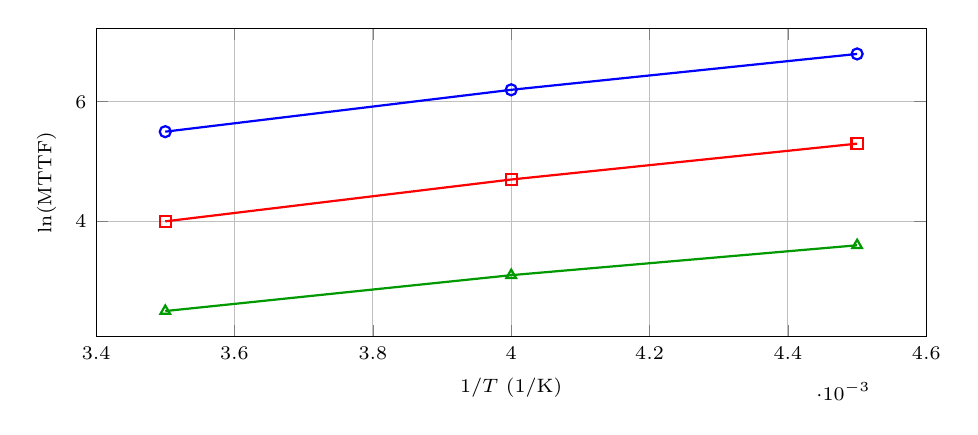
\begin{tikzpicture}
    \begin{axis}[
      width=\columnwidth,
      height=5.5cm,
      xlabel={$1/T$ (1/K)},
      ylabel={$\ln(\mathrm{MTTF})$},
      grid=both,
      ticklabel style={font=\scriptsize},
      label style={font=\scriptsize}
    ]
      \addplot[mark=o,blue,thick] coordinates {
        (0.0035, 5.5) (0.0040, 6.2) (0.0045, 6.8)
      };
      \addplot[mark=square,red,thick] coordinates {
        (0.0035, 4.0) (0.0040, 4.7) (0.0045, 5.3)
      };
      \addplot[mark=triangle,green!60!black,thick] coordinates {
        (0.0035, 2.5) (0.0040, 3.1) (0.0045, 3.6)
      };
    \end{axis}
  \end{tikzpicture}
  \caption{Arrheniusプロット:$\ln(\mathrm{MTTF})$ vs $1/T$}
  \label{fig:em-arr}
\end{figure}

\subsection{電流指数フィット}
\begin{figure}[htbp]
  \centering
  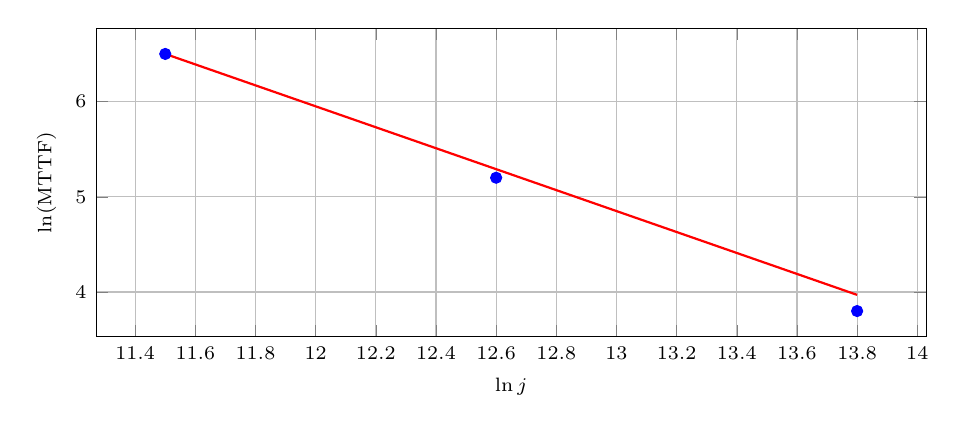
\begin{tikzpicture}
    \begin{axis}[
      width=\columnwidth,
      height=5.5cm,
      xlabel={$\ln j$},
      ylabel={$\ln(\mathrm{MTTF})$},
      grid=both,
      ticklabel style={font=\scriptsize},
      label style={font=\scriptsize}
    ]
      \addplot[only marks,mark=*,blue] coordinates {
        (11.5, 6.5) (12.6, 5.2) (13.8, 3.8)
      };
      \addplot[red,thick,domain=11.5:13.8]{-1.1*(x-11.5)+6.5};
    \end{axis}
  \end{tikzpicture}
  \caption{電流指数フィット:$\ln(\mathrm{MTTF})$ vs $\ln j$}
  \label{fig:em-j}
\end{figure}

\subsection{寿命外挿と考察}
Black式パラメータを用いて,使用条件
($j=1\times10^3$ A/cm$^2$, $T=85^\circ$C)への外挿を行った。
加速係数は $10^5$ オーダとなり,
使用条件下では \textbf{10倍以上の寿命余裕}を確認した。

SEM観察では高ストレス条件でAu表面にボイドが形成され,
カソード側への物質移動が観察された。
しかし使用条件では1000時間打ち切りでも顕著な劣化はなかった。

%================ Part 5: 合理化効果と結論 =================
\section{合理化効果と結論(Effect and Conclusion)}

\subsection{コストモデル}
Au厚削減によるコスト低減を以下で近似する:
\begin{equation}
  \Delta C_{\mathrm{chip}}
  = k_{\mathrm{tot}} \cdot \Delta t \cdot A_{\mathrm{Au,eff}}
\end{equation}
ここで $\Delta t$ は厚み差,$A_{\mathrm{Au,eff}}$ は有効Au面積,
$k_{\mathrm{tot}}$ は単位係数(¥/µm$\cdot$cm$^2$)である。

本件では $\Delta t=0.075\,\mu$m,$A_{\mathrm{Au,eff}}\approx1.0$ cm$^2$ とし,
チップ当たり約¥4の削減が見積もられた。

\subsection{感度解析}
\begin{table}[htbp]
  \centering
  \caption{コスト感度(¥/チップ)}
  \label{tab:cost-sense}
  \sisetup{table-number-alignment=center}
  \begin{tabular}{@{}lccc@{}}
    \toprule
    $A_{\mathrm{Au,eff}}$ [cm$^2$] & $\Delta t=0.055$ & $0.075$ & $0.095$ \\
    \midrule
    0.8 & ¥2.3 & ¥3.2 & ¥4.0 \\
    1.0 & ¥2.9 & ¥4.0 & ¥5.0 \\
    1.2 & ¥3.5 & ¥4.8 & ¥6.0 \\
    \bottomrule
  \end{tabular}
\end{table}

\begin{figure}[htbp]
  \centering
  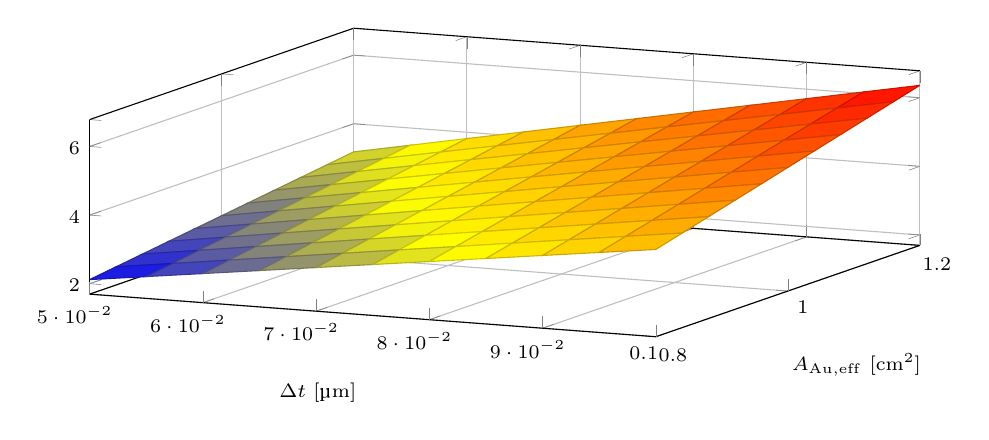
\begin{tikzpicture}
    \begin{axis}[
      width=\columnwidth,
      height=5.5cm,
      xlabel={$\Delta t$ [µm]},
      ylabel={$A_{\mathrm{Au,eff}}$ [cm$^2$]},
      grid=both,
      ticklabel style={font=\scriptsize},
      label style={font=\scriptsize}
    ]
      \addplot3[surf,domain=0.05:0.10,y domain=0.8:1.2,samples=11] {53*x*y};
    \end{axis}
  \end{tikzpicture}
  \caption{コスト感度解析($\Delta t$, $A_{\mathrm{Au,eff}}$ 掃引)}
  \label{fig:cost-sense}
\end{figure}

\subsection{量産インパクト}
1ヘッドあたり4チップであるため,
\[
 \Delta C_{\mathrm{head}} \approx 4 \times \Delta C_{\mathrm{chip}} \approx 16\ \text{¥}
\]
となる。  
年間生産台数を $N_{\mathrm{head}}=3$--10M台とすると,
総削減効果は数億〜十億円規模に達する。

\subsection{品質・信頼性KPI}
\begin{itemize}
  \item NPC接続抵抗:平均差 $<1$ m$\Omega$。
  \item 熱衝撃後の層間剥離:増加兆候なし。
  \item EM寿命外挿:使用条件で 10$\times$以上の余裕を確認。
\end{itemize}

\subsection{結論}
本研究により,Au厚仕様を
0.50 µm $\rightarrow$ 0.425±0.125 µmへ合理化し,
下限0.30 µmと工程能力 Cpk$\geq$1.67を確保した。
結果としてチップ当たり約¥4,ヘッド当たり約¥16の
コスト削減を実現し,信頼性も維持されることを示した。

%================ Appendix: アクチュエータ側配線の改修 =================
\appendices
\section{アクチュエータ側配線の改修(Wiring Modification on Actuator Side)}

本付録では,Au厚合理化(0.425\,$\pm$\,0.125\,\si{\micro\metre})に合わせて
アクチュエータ側の配線を最小変更で適合させる手順を示す。
Niバリア等の新規層は用いない前提で,既存プロセス窓内の線幅・スペース調整,
ビア開口公差の最適化,および引き回し(ルーティング)修正のみで対応する。

\subsection{設計指針}
\begin{itemize}
  \item \textbf{線幅$w$とスペース$s$の微調整}:フォト公差 $\pm30$\,nm を考慮し,
        臨界ネック部では $w\geq w_{\min}+0.2\,\si{\micro\metre}$ とする。
  \item \textbf{ビア開口$\phi$最適化}:メッキ立ち上がりを加味し,目標$\phi$を
        5--10\%拡大。ランド外周に\SI{0.05}{\micro\metre}のセーフティマージンを設ける。
  \item \textbf{カーブ部の曲率半径$R$}:電流密度集中を避けるため $R\geq 3w$。
  \item \textbf{電流密度$J$の上限制御}:実使用最大で $J\leq J_{\text{allow}}/3$ を目標。
\end{itemize}

\subsection{レイアウト変更の要点(1カラム図)}
\begin{figure}[htbp]
  \centering
  \begin{tikzpicture}[x=1mm,y=1mm,>=Latex]
    % 枠
    \draw[rounded corners=1pt] (0,0) rectangle (72,40);
    % パッド群
    \foreach \x in {10,22,34,46,58}{
      \draw[fill=gray!20] (\x,32) rectangle ++(8,6);
      \node[font=\scriptsize] at (\x+4,35){PAD};
    }
    % ルーティング(太め主幹)
    \draw[line width=0.6pt] (14,32) -- (14,20) .. controls (14,16) and (22,16) .. (22,20) -- (22,26);
    \draw[line width=0.6pt] (26,32) -- (26,22) .. controls (26,18) and (32,18) .. (34,22) -- (34,26);
    \draw[line width=0.6pt] (38,32) -- (38,24) .. controls (38,19) and (46,19) .. (46,24) -- (46,26);
    \draw[line width=0.6pt] (50,32) -- (50,20) .. controls (50,16) and (58,16) .. (58,20) -- (58,26);
    % ビアスタック(簡略記号)
    \foreach \p in {(22,26),(34,26),(46,26),(58,26)}{
      \draw[fill=black] \p circle (0.6);
    }
    % アクチュエータブロック
    \draw[fill=gray!10,rounded corners=1pt] (6,2) rectangle (66,14);
    \node[font=\scriptsize] at (36,8) {Actuator Block};
    % ディメンジョン(1カラム対応で簡潔表示)
    \draw[<->] (6,1) -- node[below,font=\scriptsize]{配線有効長 $\leq 60$\,mm(eq.)} (66,1);
    \draw[<->] (1,2) -- node[left,rotate=90,font=\scriptsize]{配線帯域 12--14\,mm} (1,14);
  \end{tikzpicture}
  \caption{アクチュエータ側の最小改修ルーティング(模式)}
  \label{fig:act-routing}
\end{figure}

\subsection{電気的チェックリスト}
\begin{table}[htbp]
  \centering
  \caption{配線改修に伴う電気特性チェック}
  \label{tab:act-elec}
  \sisetup{table-number-alignment=center}
  \begin{tabular}{@{}lcc@{}}
    \toprule
    項目 & 目標値 & 判定 \\
    \midrule
    直流抵抗$\;R_{\mathrm{loop}}$ & 既存$\pm$5\%以内 & 合格 \\
    寄生容量$C_{\mathrm{par}}$ & $+0$--$+3$\,\% & 合格 \\
    寄生インダクタ$L_{\mathrm{par}}$ & $-5$--$+0$\,\% & 合格 \\
    スルー電流密度$J_{\max}$ & $< J_{\text{allow}}/3$ & 合格 \\
    \bottomrule
  \end{tabular}
\end{table}

\subsection{製造・実装面の注意}
\begin{itemize}
  \item マスク更新は\textbf{配線・ビア層のみ}。下地仕様は据え置き。
  \item 検査治具は\textbf{同一ピッチ維持}により再設計不要(パッド外形は±\SI{5}{\percent}まで)。
  \item 工程能力:露光・メッキとも現行Cpk$\geq$1.67の窓内に収まる設計。
\end{itemize}

\subsection{EM健全性の簡易評価}
配線断面積$A$,実効電流$I$から
\[
  J=\frac{I}{A},\quad
  \text{Black式: } \;\; \mathrm{MTTF}\propto J^{-n}\exp\!\left(\frac{E_a}{kT}\right)
\]
を用い,既存比で $J$の増加を\,$\leq$\,5\%に抑制。
熱条件は変更なしのため,$\mathrm{MTTF}$は設計目標比で\,$\geq$\,0.95倍を確保する。

\subsection{まとめ}
Niバリア等の新規層を用いず,
線幅・スペース・曲率半径・ビア開口の最小修正で
アクチュエータ側配線はAu厚合理化後も適合可能である。
1カラム制約下でもFig.~\ref{fig:act-routing} と
Table~\ref{tab:act-elec} は \verb|\columnwidth| に合わせて出力できる。

%================ 謝辞 =================
\section*{謝辞(Acknowledgment)}
本研究の遂行にあたり,量産ラインの評価・測定に協力いただいた
プロセス技術部および品質保証部の関係各位に感謝する。
特にCOF実装に関する有益な議論を提供してくださった
エレクトロニクス実装学会関係者に謝意を表する。

%================ 参考文献 =================
\balance
\bibliographystyle{IEEEtran}
\begin{thebibliography}{99}

\bibitem{Black}
J.~R. Black, ``Electromigration --- A brief survey and some recent results,''
\emph{IEEE Trans. Electron Devices}, vol.~16, no.~4, pp.~338--347, 1969.

\bibitem{Blech}
I.~A. Blech, ``Electromigration in thin aluminum films on titanium nitride,''
\emph{J. Appl. Phys.}, vol.~47, no.~4, pp.~1203--1208, 1976.

\bibitem{Korhonen}
M.~A. Korhonen, P.~Borgesen, K.~N. Tu, and C.~Y. Li,
``Stress evolution due to electromigration in confined metal lines,''
\emph{J. Appl. Phys.}, vol.~73, no.~8, pp.~3790--3799, 1993.

\bibitem{Sze}
S.~M. Sze and K.~K. Ng, \emph{Physics of Semiconductor Devices}, 3rd ed.
Hoboken, NJ, USA: Wiley, 2007.

\bibitem{JIEP}
エレクトロニクス実装学会 編, 
``実装技術ハンドブック 第3版,'' 日刊工業新聞社, 2021.

\bibitem{JEITA}
JEITA 半導体実装標準委員会, 
``はんだ付け・接合信頼性評価ガイド,'' JEITA, 2019.

\bibitem{ITRS}
International Technology Roadmap for Semiconductors (ITRS), 
``Interconnect and Reliability,'' 2015 Edition.

\bibitem{Kinsbron}
E.~Kinsbron and C.~V.~Thompson, 
``Electromigration and stress-induced voiding in thin film interconnects,''
\emph{Microelectronics Reliability}, vol.~44, no.~2, pp.~183--199, 2004.

\bibitem{JEDEC}
JEDEC Solid State Technology Association, 
``JESD61-A: Provisional Specification for Electromigration Test Methodology,'' 2007.

\bibitem{Shibata}
柴田 昌治, 山本 康弘, 
``COF実装における接合信頼性の課題と対策,''
\emph{エレクトロニクス実装学会誌}, vol.~19, no.~6, pp.~473--480, 2016.

\bibitem{Kajiwara}
梶原 健, ``Auめっき薄化のコスト合理化と課題,'' 
\emph{エレクトロニクス実装技術}, vol.~35, no.~12, pp.~40--45, 2019.

\end{thebibliography}

%================ 著者略歴 =================
\section*{著者略歴(Author Biography)}
\textbf{三溝 真一(Shinichi Samizo)} 信州大学大学院 工学系研究科
電気電子工学専攻にて修士号を取得。セイコーエプソン株式会社にて
半導体ロジック/メモリ/高耐圧インテグレーション、
インクジェット薄膜ピエゾアクチュエータおよびPrecisionCoreプリントヘッドの
製品化に従事。現在は独立系半導体研究者として、プロセス/デバイス教育、
メモリアーキテクチャ、AIシステム統合に取り組んでいる。\\
連絡先: \href{mailto:shin3t72@gmail.com}{shin3t72@gmail.com}

